\scanpage{25}
\deleted{Soit en effet} Si on a $U_s\subset % BEGIN B025-S01
% proposal: \deleted{\unsure{E|I}}\Sigma_{\unsure{i|\prime}}^-
% qualification: Old E/I; short undotted index i/prime; detached upper run head or retrace/independent run. First occurrence carries the recurring head and index qualification.
% complete candidates: \deleted{E}\Sigma_i^- || \deleted{I}\Sigma_i^- || \deleted{E}\Sigma_{\prime}^- || \deleted{I}\Sigma_{\prime}^-
% ownership: Complete overwritten first Sigma, its surviving predecessor strokes, detached upper run, minus and one short index stroke; comma remains outside.
% complete upper-run role candidates: head/retrace of this complete Sigma; independent upper run adjoining this complete Sigma. Main glyph his hand; independent-run hand undetermined.
\mathord{\unsure{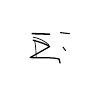
\begin{tikzpicture}[x=0.018em,y=-0.018em,baseline=(base),line cap=round,line join=round]
\path[use as bounding box] (0,0) rectangle (94,75);
\coordinate (base) at (0,61);
\begin{scope}[shift={(-830,-119)}]
\node[overlay,anchor=base west,inner sep=0pt,outer sep=0pt] at (830,180) {$\phantom{\deleted{\unsure{E|I}}\Sigma_{\unsure{i|\prime}}^-}$};
\draw[line width=.055em] (839,131) -- (874,132);
\draw[line width=.025em] (841,138) .. controls (853,140) and (865,146) .. (873,154);
\draw[line width=.045em] (841,144) .. controls (854,148) and (868,152) .. (874,157) -- (835,179) .. controls (856,180) and (881,178) .. (893,182) -- (895,190);
\draw[line width=.026em] (844,145) .. controls (846,155) and (847,168) .. (847,177);
\draw[line width=.040em] (896,129) -- (914,131);
\draw[line width=.036em] (901,158) -- (906,165);
\end{scope}
\end{tikzpicture}}}
% END B025-S01
$, $\overline{U_s}% BEGIN B025-G02
% proposal: \deleted{\unsure{=}}\cap E_{\unsure{i|j}}
% qualification: The overwritten equals candidate and the i/j index remain independently qualified.
% complete candidates: \deleted{=}\cap E_i || \deleted{=}\cap E_j || \cap E_i || \cap E_j
% ownership: Overwritten relation plus E and its complete two-part index. U-bar, non-equality, empty-set sign and comma remain outside.
\mathord{\unsure{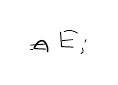
\begin{tikzpicture}[x=0.018em,y=-0.018em,baseline=(base),line cap=round,line join=round]
\path[use as bounding box] (0,0) rectangle (125,58);
\coordinate (base) at (0,45);
\begin{scope}[shift={(-1100,-133)}]
\node[overlay,anchor=base west,inner sep=0pt,outer sep=0pt] at (1100,178) {$\phantom{\deleted{\unsure{=}}\cap E_{\unsure{i|j}}}$};
\draw[line width=.032em] (1106,168) -- (1135,166);
\draw[line width=.030em] (1106,176) -- (1110,176);
\draw[line width=.037em] (1113,175) -- (1136,176);
\draw[line width=.053em] (1113,174) .. controls (1123,153) and (1136,155) .. (1140,174) -- (1140,181);
\draw[line width=.035em] (1166,142) -- (1168,171) -- (1191,172);
\draw[line width=.029em] (1173,141) .. controls (1182,136) and (1193,139) .. (1200,144);
\draw[line width=.030em] (1169,159) -- (1190,157);
\draw[line width=.030em] (1217,157) -- (1215,162);
\draw[line width=.030em] (1210,174) .. controls (1213,183) and (1210,184) .. (1207,185);
\end{scope}
\end{tikzpicture}}}
% END B025-G02
\ne\varnothing$, \deleted{et si} alors $% BEGIN B025-G03
% proposal: \text{on a}
% qualification: Reduced on a primary; the three visible marks also permit an unassigned three-mark group.
% complete candidates: on a || three unassigned marks
% ownership: Entire reduced on a continuation, consisting of three marks. The preceding alors remains outside.
\mathord{\unsure{\begin{tikzpicture}[x=0.018em,y=-0.018em,baseline=(base),line cap=round,line join=round]
\path[use as bounding box] (0,0) rectangle (143,21);
\coordinate (base) at (0,16);
\begin{scope}[shift={(-296,-283)}]
\node[overlay,anchor=base west,inner sep=0pt,outer sep=0pt] at (296,299) {$\phantom{\text{on a}}$};
\fill (301,295) -- (304,293) -- (306,296) -- (302,299) -- cycle;
\draw[line width=.023em] (328,296) .. controls (337,294) and (349,290) .. (356,295);
\draw[line width=.030em] (424,295) .. controls (428,292) and (432,293) .. (435,295);
\end{scope}
\end{tikzpicture}}}
% END B025-G03
$
\[
\begin{aligned}
U_s=X\setminus % BEGIN B025-G04
% proposal: \mathop{\unsure{\rlap{\raisebox{.65ex}{$\scriptstyle-$}}\bigcup|\deleted{\bigcap}\bigcup}}\limits_{\alpha\in K}
% qualification: Union with a high cross and doubled bowl; union over earlier intersection remains the complete state alternative.
% complete candidates: \mathop{\rlap{\raisebox{.65ex}{$\scriptstyle-$}}\bigcup}\limits_{\alpha\in K} || \mathop{\deleted{\bigcap}\bigcup}\limits_{\alpha\in K}
% ownership: Complete large operator, high transverse run, upper-left curved return, doubled bowl and alpha-in-K limit, each once.
\mathord{\unsure{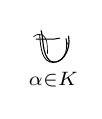
\begin{tikzpicture}[x=0.018em,y=-0.018em,baseline=(base),line cap=round,line join=round]
\path[use as bounding box] (0,0) rectangle (93,126);
\coordinate (base) at (0,71);
\begin{scope}[shift={(-838,-269)}]
\node[overlay,anchor=base west,inner sep=0pt,outer sep=0pt] at (838,340) {$\phantom{\mathop{\unsure{\rlap{\raisebox{.65ex}{$\scriptstyle-$}}\bigcup|\deleted{\bigcap}\bigcup}}\limits_{\alpha\in K}}$};
\draw[line width=.024em] (850,287) .. controls (862,277) and (875,283) .. (877,302) -- (878,321);
\draw[line width=.042em] (865,275) .. controls (870,289) and (866,322) .. (883,336) .. controls (905,347) and (926,314) .. (920,286);
\draw[line width=.030em] (862,283) .. controls (864,311) and (867,338) .. (889,339) .. controls (911,337) and (920,316) .. (915,291);
\draw[line width=.037em] (855,292) .. controls (872,291) and (889,294) .. (902,290);
\draw[line width=.020em] (915,292) -- (918,302);
\node[anchor=base west,inner sep=0pt,outer sep=0pt] at (840,386) {$\scriptstyle\alpha\in K$};
\end{scope}
\end{tikzpicture}}}
% END B025-G04
% BEGIN B025-S02
% proposal: \widehat{\Sigma}_\alpha^+
% qualification: The two tiny intervening traces have unresolved alpha/plus-retrace or independent-mark attachment, hand and surface origin.
% complete candidates: Hatted Sigma-alpha-plus with both traces attached to local writing || Hatted Sigma-alpha-plus with one or both traces independent
% ownership: Complete hatted Sigma with joined head, alpha, plus, and the two small traces between plus and alpha. No separate copy of either mark.
\mathord{\unsure{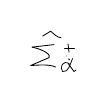
\begin{tikzpicture}[x=0.018em,y=-0.018em,baseline=(base),line cap=round,line join=round]
\path[use as bounding box] (0,0) rectangle (103,97);
\coordinate (base) at (0,80);
\begin{scope}[shift={(-965,-253)}]
\node[overlay,anchor=base west,inner sep=0pt,outer sep=0pt] at (965,333) {$\phantom{\widehat{\Sigma}_\alpha^+}$};
\draw[line width=.030em] (974,292) -- (1018,287);
\draw[line width=.031em] (974,292) .. controls (1000,298) and (1012,308) .. (1008,313) -- (971,329) .. controls (988,328) and (1008,326) .. (1021,332);
\draw[line width=.029em] (995,270) -- (1011,260) .. controls (1019,267) and (1025,273) .. (1032,273);
\draw[line width=.031em] (1046,286) -- (1048,302);
\draw[line width=.031em] (1039,294) -- (1059,294);
\draw[line width=.027em] (1049,326) .. controls (1036,316) and (1028,333) .. (1035,341) .. controls (1047,344) and (1051,324) .. (1055,315);
\draw[line width=.030em] (1047,326) -- (1058,341) -- (1062,338);
\draw[line width=.015em,gray] (1042,309) -- (1044,311);
\fill (1046,315) -- (1050,316) -- (1048,319) -- cycle;
\end{scope}
\end{tikzpicture}}}
% END B025-S02
&\qquad\text{où}\quad i\in K\subset I\\
&\forall\alpha\in K\qquad % BEGIN B025-S03
% proposal: \Sigma_\alpha^+
% ownership: Complete condition Sigma, locally joined top arm, alpha and plus.
\mathord{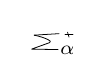
\begin{tikzpicture}[x=0.018em,y=-0.018em,baseline=(base),line cap=round,line join=round]
\path[use as bounding box] (0,0) rectangle (102,56);
\coordinate (base) at (0,44);
\begin{scope}[shift={(-1240,-354)}]
\node[overlay,anchor=base west,inner sep=0pt,outer sep=0pt] at (1240,398) {$\phantom{\Sigma_\alpha^+}$};
\draw[line width=.028em] (1253,369) -- (1303,366);
\draw[line width=.029em] (1253,369) .. controls (1277,374) and (1291,382) .. (1284,384) -- (1248,397) -- (1301,398);
\draw[line width=.026em] (1320,363) -- (1323,373);
\draw[line width=.026em] (1315,367) -- (1331,367);
\node[anchor=base west,inner sep=0pt,outer sep=0pt] at (1305,407) {$\scriptstyle\alpha$};
\end{scope}
\end{tikzpicture}}
% END B025-S03
\in\pi_0(X\setminus E_\alpha)\ % BEGIN B025-G05
% proposal: \deleted{\unsure{\text{les}|K|\text{tel}}}
% qualification: Deleted les/K/tel remain supported; the crossed cluster has no separately visible endpoint comma.
% complete candidates: \deleted{\text{les}} || \deleted{K} || \deleted{\text{tel}}
% ownership: Whole terminal deleted cluster and its crossing, with no added comma.
\mathord{\unsure{
\begin{tikzpicture}[x=0.018em,y=-0.018em,baseline=(base),line cap=round,line join=round]
\path[use as bounding box] (0,0) rectangle (76,57);
\coordinate (base) at (0,45);
\begin{scope}[shift={(-1597,-342)}]
\node[overlay,anchor=base west,inner sep=0pt,outer sep=0pt] at (1597,387) {$\phantom{\deleted{\unsure{\text{les}|K|\text{tel}}}}$};
\draw[line width=.028em] (1611,350) -- (1613,385) .. controls (1618,380) and (1626,370) .. (1632,356);
\draw[line width=.029em] (1606,367) -- (1633,351) .. controls (1636,361) and (1626,369) .. (1616,370);
\draw[line width=.026em] (1622,373) .. controls (1625,385) and (1637,383) .. (1642,372);
\draw[line width=.027em] (1646,367) -- (1642,387);
\draw[line width=.034em] (1625,381) -- (1665,379);
\end{scope}
\end{tikzpicture}}}
% END B025-G05
\\
&% BEGIN B025-G06
% proposal: \unsure{\deleted{U\Sigma}|\deleted{\bigcup\Sigma}|\deleted{U}|U\Sigma}
% qualification: Original whole-cluster glyph alternatives retained; separate cancellation/live-state qualification added.
% complete candidates: \deleted{U\Sigma} || \deleted{\bigcup\Sigma} || \deleted{U} || U\Sigma
% ownership: Complete bowl, inner angular form and descending return before les; les remains outside.
\mathord{\unsure{
\begin{tikzpicture}[x=0.018em,y=-0.018em,baseline=(base),line cap=round,line join=round]
\path[use as bounding box] (0,0) rectangle (60,74);
\coordinate (base) at (0,53);
\begin{scope}[shift={(-1103,-439)}]
\node[overlay,anchor=base west,inner sep=0pt,outer sep=0pt] at (1103,492) {$\phantom{\unsure{\deleted{U\Sigma}|\deleted{\bigcup\Sigma}|\deleted{U}|U\Sigma}}$};
\draw[line width=.024em] (1112,450) .. controls (1112,479) and (1113,498) .. (1131,499) .. controls (1148,496) and (1154,465) .. (1150,449);
\draw[line width=.023em] (1118,459) -- (1149,449) -- (1132,475) -- (1150,476);
\draw[line width=.033em] (1150,450) .. controls (1153,473) and (1148,487) .. (1137,503) .. controls (1142,511) and (1152,505) .. (1156,501);
\end{scope}
\end{tikzpicture}}}
% END B025-G06
\ \text{les }% BEGIN B025-S04
% proposal: \Sigma_\alpha^+
% complete candidates: Sigma-alpha-plus with head/retrace || Sigma-alpha-plus with independent upper run
% ownership: Complete disjointness Sigma, separate upper head run, alpha and plus; recurring head-role qualification is first printed in S01.
% complete upper-run role candidates: head/retrace of this complete Sigma; independent upper run adjoining this complete Sigma. Main glyph his hand; independent-run hand undetermined.
\mathord{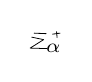
\begin{tikzpicture}[x=0.018em,y=-0.018em,baseline=(base),line cap=round,line join=round]
\path[use as bounding box] (0,0) rectangle (73,53);
\coordinate (base) at (0,41);
\begin{scope}[shift={(-1287,-433)}]
\node[overlay,anchor=base west,inner sep=0pt,outer sep=0pt] at (1287,474) {$\phantom{\Sigma_\alpha^+}$};
\draw[line width=.030em] (1300,444) -- (1324,445);
\draw[line width=.028em] (1295,452) -- (1319,457) -- (1292,474) -- (1326,475);
\draw[line width=.029em] (1345,441) -- (1346,453);
\draw[line width=.029em] (1337,446) -- (1352,444);
\node[anchor=base west,inner sep=0pt,outer sep=0pt] at (1324,482) {$\scriptstyle\alpha$};
\end{scope}
\end{tikzpicture}}
% END B025-S04
\ \text{mut\textsuperscript{t}. disjoints}
\end{aligned}
\]

Il faut voir que $% BEGIN B025-G07
% proposal: \deleted{K}\inserted{K\setminus\{i\}}
% ownership: Raised replacement K-setminus-braced-i, deleted K and its crossing/long bent guide; following et remains outside.
\mathord{
\begin{tikzpicture}[x=0.018em,y=-0.018em,baseline=(base),line cap=round,line join=round]
\path[use as bounding box] (0,0) rectangle (189,159);
\coordinate (base) at (0,132);
\begin{scope}[shift={(-876,-481)}]
\node[overlay,anchor=base west,inner sep=0pt,outer sep=0pt] at (876,613) {$\phantom{\deleted{K}\inserted{K\setminus\{i\}}}$};
\draw[line width=.029em] (881,488) .. controls (889,506) and (885,528) .. (895,536);
\draw[line width=.029em] (915,493) .. controls (919,510) and (897,523) .. (889,528) -- (913,545);
\draw[line width=.033em] (927,519) -- (940,535);
\draw[line width=.026em] (958,504) -- (956,525) -- (963,528) -- (965,545);
\draw[line width=.026em] (994,504) .. controls (985,525) and (999,523) .. (1000,536) -- (992,544);
\draw[line width=.023em] (974,518) -- (978,531);
\draw[line width=.027em] (978,502) -- (980,506);
\draw[line width=.028em] (959,551) -- (972,619);
\draw[line width=.029em] (978,552) -- (995,550) -- (965,575);
\draw[line width=.030em] (999,561) .. controls (1016,563) and (997,582) .. (986,594) -- (1001,610);
\draw[line width=.034em] (973,597) -- (1003,617);
\draw[line width=.034em] (1002,583) .. controls (997,600) and (982,620) .. (976,632);
\draw[line width=.019em] (925,622) .. controls (911,590) and (958,571) .. (1058,530) .. controls (1062,528) and (1062,527) .. (1056,529);
\end{scope}
\end{tikzpicture}}
% END B025-G07
$ et les $% BEGIN B025-S05
% proposal: \Sigma_\alpha^+
% complete candidates: Sigma-alpha-plus with head/retrace || Sigma-alpha-plus with independent upper run
% ownership: Complete prose Sigma with detached upper head, alpha and plus; parenthetical condition remains outside.
% complete upper-run role candidates: head/retrace of this complete Sigma; independent upper run adjoining this complete Sigma. Main glyph his hand; independent-run hand undetermined.
\mathord{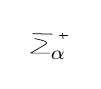
\begin{tikzpicture}[x=0.018em,y=-0.018em,baseline=(base),line cap=round,line join=round]
\path[use as bounding box] (0,0) rectangle (90,67);
\coordinate (base) at (0,52);
\begin{scope}[shift={(-1234,-548)}]
\node[overlay,anchor=base west,inner sep=0pt,outer sep=0pt] at (1234,600) {$\phantom{\Sigma_\alpha^+}$};
\draw[line width=.028em] (1244,560) -- (1283,561);
\draw[line width=.024em] (1248,570) .. controls (1269,574) and (1277,577) .. (1269,582) -- (1240,599) -- (1278,599);
\draw[line width=.027em] (1304,559) -- (1305,570);
\draw[line width=.027em] (1298,563) -- (1314,563);
\node[anchor=base west,inner sep=0pt,outer sep=0pt] at (1280,612) {$\scriptstyle\alpha$};
\end{scope}
\end{tikzpicture}}
% END B025-S05
$ $(\alpha\in K\setminus\{i\})$ sont \unsure{determinés|déterminés|determines} en termes de $i$ et de $% BEGIN B025-S06
% proposal: \Sigma_i^+
% complete candidates: \Sigma_i^+ || \Sigma_{\prime}^+
% ownership: Complete signed plus Sigma, detached head, plus and one short index stroke; i/prime and head-role doubts recur from S01.
% complete upper-run role candidates: head/retrace of this complete Sigma; independent upper run adjoining this complete Sigma. Main glyph his hand; independent-run hand undetermined.
\mathord{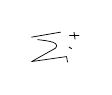
\begin{tikzpicture}[x=0.018em,y=-0.018em,baseline=(base),line cap=round,line join=round]
\path[use as bounding box] (0,0) rectangle (113,79);
\coordinate (base) at (0,66);
\begin{scope}[shift={(-291,-816)}]
\node[overlay,anchor=base west,inner sep=0pt,outer sep=0pt] at (291,882) {$\phantom{\Sigma_i^+}$};
\draw[line width=.027em] (299,835) -- (357,825);
\draw[line width=.026em] (311,840) .. controls (338,843) and (355,846) .. (347,857) -- (299,884) -- (369,874) -- (371,885);
\draw[line width=.029em] (384,825) -- (386,839);
\draw[line width=.029em] (375,831) -- (394,831);
\draw[line width=.031em] (374,855) -- (379,858);
\end{scope}
\end{tikzpicture}}
% END B025-S06
$ i.e. $% BEGIN B025-S07
% proposal: \Sigma_i^-
% complete candidates: \Sigma_i^- || \Sigma_{\prime}^-
% ownership: Complete signed minus Sigma, detached head, minus and single short index; sentence full stop remains outside.
% complete upper-run role candidates: head/retrace of this complete Sigma; independent upper run adjoining this complete Sigma. Main glyph his hand; independent-run hand undetermined.
\mathord{\begin{tikzpicture}[x=0.018em,y=-0.018em,baseline=(base),line cap=round,line join=round]
\path[use as bounding box] (0,0) rectangle (100,73);
\coordinate (base) at (0,58);
\begin{scope}[shift={(-550,-805)}]
\node[overlay,anchor=base west,inner sep=0pt,outer sep=0pt] at (550,863) {$\phantom{\Sigma_i^-}$};
\draw[line width=.026em] (556,821) -- (595,817);
\draw[line width=.025em] (556,833) .. controls (579,833) and (599,837) .. (589,846) -- (563,861) .. controls (589,853) and (606,858) .. (614,865);
\draw[line width=.030em] (620,814) -- (641,814);
\draw[line width=.032em] (616,853) -- (617,856);
\end{scope}
\end{tikzpicture}}
% END B025-S07
$. Je dis $% BEGIN B025-G09
% proposal: \text{que}
% qualification: Only the small point beside q has unresolved role, hand, attachment and surface origin; que itself is firm.
% complete candidates: que with an unassigned small point beside its q descender
% ownership: Complete final que, its long q descender, and one separate small point at its right. Je dis remains outside; no additional que or point is printed.
\mathord{\unsure{\begin{tikzpicture}[x=0.018em,y=-0.018em,baseline=(base),line cap=round,line join=round]
\path[use as bounding box] (0,0) rectangle (108,113);
\coordinate (base) at (0,30);
\begin{scope}[shift={(-1050,-798)}]
\node[overlay,anchor=base west,inner sep=0pt,outer sep=0pt] at (1050,828) {$\phantom{\text{que}}$};
\draw[line width=.025em] (1063,811) .. controls (1052,802) and (1052,822) .. (1070,823) .. controls (1082,822) and (1086,818) .. (1088,809);
\draw[line width=.025em] (1068,809) .. controls (1075,817) and (1076,849) .. (1079,875) .. controls (1085,902) and (1083,906) .. (1072,903);
\draw[line width=.026em] (1088,809) .. controls (1098,820) and (1116,817) .. (1118,805) .. controls (1124,813) and (1138,811) .. (1147,813) .. controls (1152,814) and (1150,820) .. (1148,821);
\fill (1094,841) -- (1096,840) -- (1096,843) -- cycle;
\end{scope}
\end{tikzpicture}}}
% END B025-G09
$
\[
K\setminus\{i\}=% BEGIN B025-G08
% proposal: \bigl\{
% ownership: Only the final set left brace, upper and lower arms meeting at the left cusp; alpha and condition follow outside.
\mathord{\begin{tikzpicture}[x=0.018em,y=-0.018em,baseline=(base),line cap=round,line join=round]
\path[use as bounding box] (0,0) rectangle (40,118);
\coordinate (base) at (0,64);
\begin{scope}[shift={(-758,-917)}]
\node[overlay,anchor=base west,inner sep=0pt,outer sep=0pt] at (758,981) {$\phantom{\bigl\{}$};
\draw[line width=.021em] (776,925) .. controls (777,944) and (780,963) .. (779,973) .. controls (775,979) and (769,974) .. (764,974);
\draw[line width=.030em] (764,974) .. controls (783,975) and (781,1006) .. (785,1024) .. controls (790,1032) and (793,1030) .. (795,1031);
\end{scope}
\end{tikzpicture}}
% END B025-G08
\alpha\in I\mid E_\alpha\subset % BEGIN B025-S08
% proposal: \Sigma_\alpha^-
% ownership: Final Sigma-alpha-minus with locally joined thin head return; no closing brace or punctuation is included.
\mathord{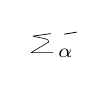
\begin{tikzpicture}[x=0.018em,y=-0.018em,baseline=(base),line cap=round,line join=round]
\path[use as bounding box] (0,0) rectangle (109,64);
\coordinate (base) at (0,53);
\begin{scope}[shift={(-1166,-899)}]
\node[overlay,anchor=base west,inner sep=0pt,outer sep=0pt] at (1166,952) {$\phantom{\Sigma_\alpha^-}$};
\draw[line width=.025em] (1177,916) -- (1212,911);
\draw[line width=.022em] (1177,916) .. controls (1191,920) and (1212,921) .. (1208,928) -- (1173,949) -- (1217,949);
\draw[line width=.030em] (1240,912) -- (1264,908);
\node[anchor=base west,inner sep=0pt,outer sep=0pt] at (1227,959) {$\scriptstyle\alpha$};
\end{scope}
\end{tikzpicture}}
% END B025-S08
\]
% Lower-sheet detached marks, in their own source positions; no lexical role assigned.
\figure{\begin{tikzpicture}[x=0.01em,y=-0.01em]
\path[use as bounding box] (0,0) rectangle (1685,1261);
\node[anchor=base west,inner sep=0pt,outer sep=0pt] at (448,252) {$% BEGIN B025-M01
% proposal: 
% qualification: Faint curved surface trace, no character assigned; role, hand and surface origin undetermined.
% ownership: Faint upper curve, pale middle continuation, lower diagonal/foot and detached left foot run.
\mathord{\unsure{\begin{tikzpicture}[x=0.01em,y=-0.01em,baseline=(base),line cap=round,line join=round]
\path[use as bounding box] (0,0) rectangle (38,44);
\coordinate (base) at (0,44);
\begin{scope}[shift={(-448,-1308)}]
\draw[line width=.013em,gray] (471,1312) .. controls (477,1315) and (480,1323) .. (480,1333);
\draw[line width=.009em,gray] (480,1333) -- (480,1338);
\draw[line width=.012em,gray] (479,1340) -- (471,1347) -- (460,1347);
\draw[line width=.007em,gray] (456,1347) -- (450,1346);
\end{scope}
\end{tikzpicture}}}
% END B025-M01
$};
\node[anchor=base west,inner sep=0pt,outer sep=0pt] at (1592,630) {$% BEGIN B025-M02
% proposal: 
% qualification: Two dark diagonal points; character, role, hand and surface origin undetermined.
% ownership: Both isolated lower-right points, with no colon or other character supplied.
\mathord{\unsure{\begin{tikzpicture}[x=0.01em,y=-0.01em,baseline=(base),line cap=round,line join=round]
\path[use as bounding box] (0,0) rectangle (14,17);
\coordinate (base) at (0,17);
\begin{scope}[shift={(-1592,-1713)}]
\fill (1600,1718) ellipse [x radius=1.4,y radius=1.8];
\fill (1595,1725) ellipse [x radius=1.7,y radius=1.6];
\end{scope}
\end{tikzpicture}}}
% END B025-M02
$};
\end{tikzpicture}}
% archive sheet number: 24
